\section{Insights into LLM Serving Systems}
\label{sec:analysis}

To understand the memory allocation pattern of LLM serving systems, we experiment with  \yismall running on a single A100 GPU, and \llamasmall and \yimedium running on two A100 GPUs with tensor-parallelism (TP). We set the initial context length of each request to 1K tokens, vary the batch size from 1 to 320 and measure the throughput and memory requirement of the decode phase (see \autoref{sec:design:optimizations} for our discussion and optimizations for the prefill phase).




\noindent
\textbf{Observation-1:} \textit{\kvcache memory requirement is predictable on a per-iteration basis}. Due to auto-regressive decoding, once a request enters the decode phase, its \kvcache size increases uniformly by one token per iteration. This allows the serving system to determine in advance if additional memory will be required during the iteration's execution.\footnote{Note that this prediction is possible only at the granularity of individual iterations; the total \kvcache requirement of a request remains unknown as it depends on the total number of output tokens in the request.}


\noindent
\textbf{Observation-2:} \textit{\kvcache does not require high memory allocation bandwidth.} The memory footprint of a single token across all layers is typically few 10s-100s of kilobytes of memory. For example, the per-token memory footprint of \yismall, \llamasmall and \yimedium is 64KB, 128KB and 240KB, respectively. Further, each iteration runs for 10s-100s of milliseconds implying that a request requires at most a few megabytes of memory per second. While batching improves system throughput~\cite{sarathi2023,sarathiserve2024,patel2023splitwise,distserve2024}, the number of tokens generated per second plateaus beyond a certain batch size (\autoref{fig:analysis:llm:memory:top}). This implies that the memory allocation bandwidth requirement also saturates at large batch sizes (e.g., at 256 for \yimedium). For all the models we studied, we observe that the highest memory allocation rate is at most 750MB per second (\autoref{fig:analysis:llm:memory:bottom}). \sysname leverages these observations to optimize \kvcache memory management. 


\begin{figure}[t]
    \centering
    \begin{subfigure}[b]{0.9\columnwidth}
    \centering
        %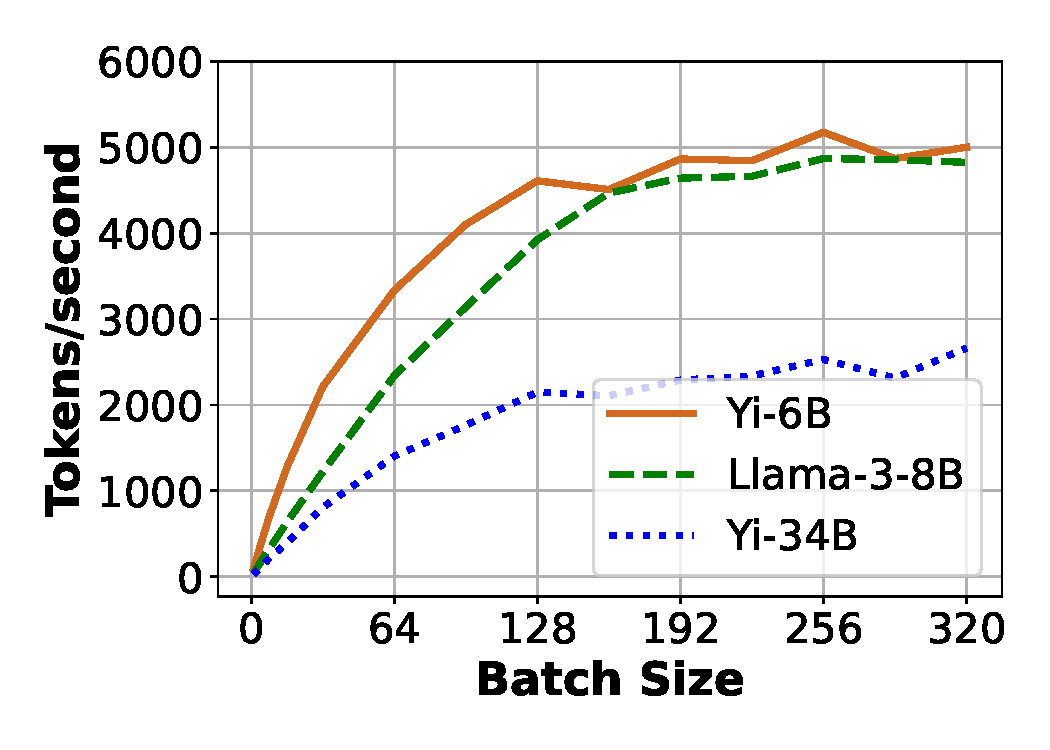
\includegraphics[trim={0 25 0 0}, clip=True, width=\textwidth]{graphs/analysis_decode_throughput/analysis_throughput.pdf}
        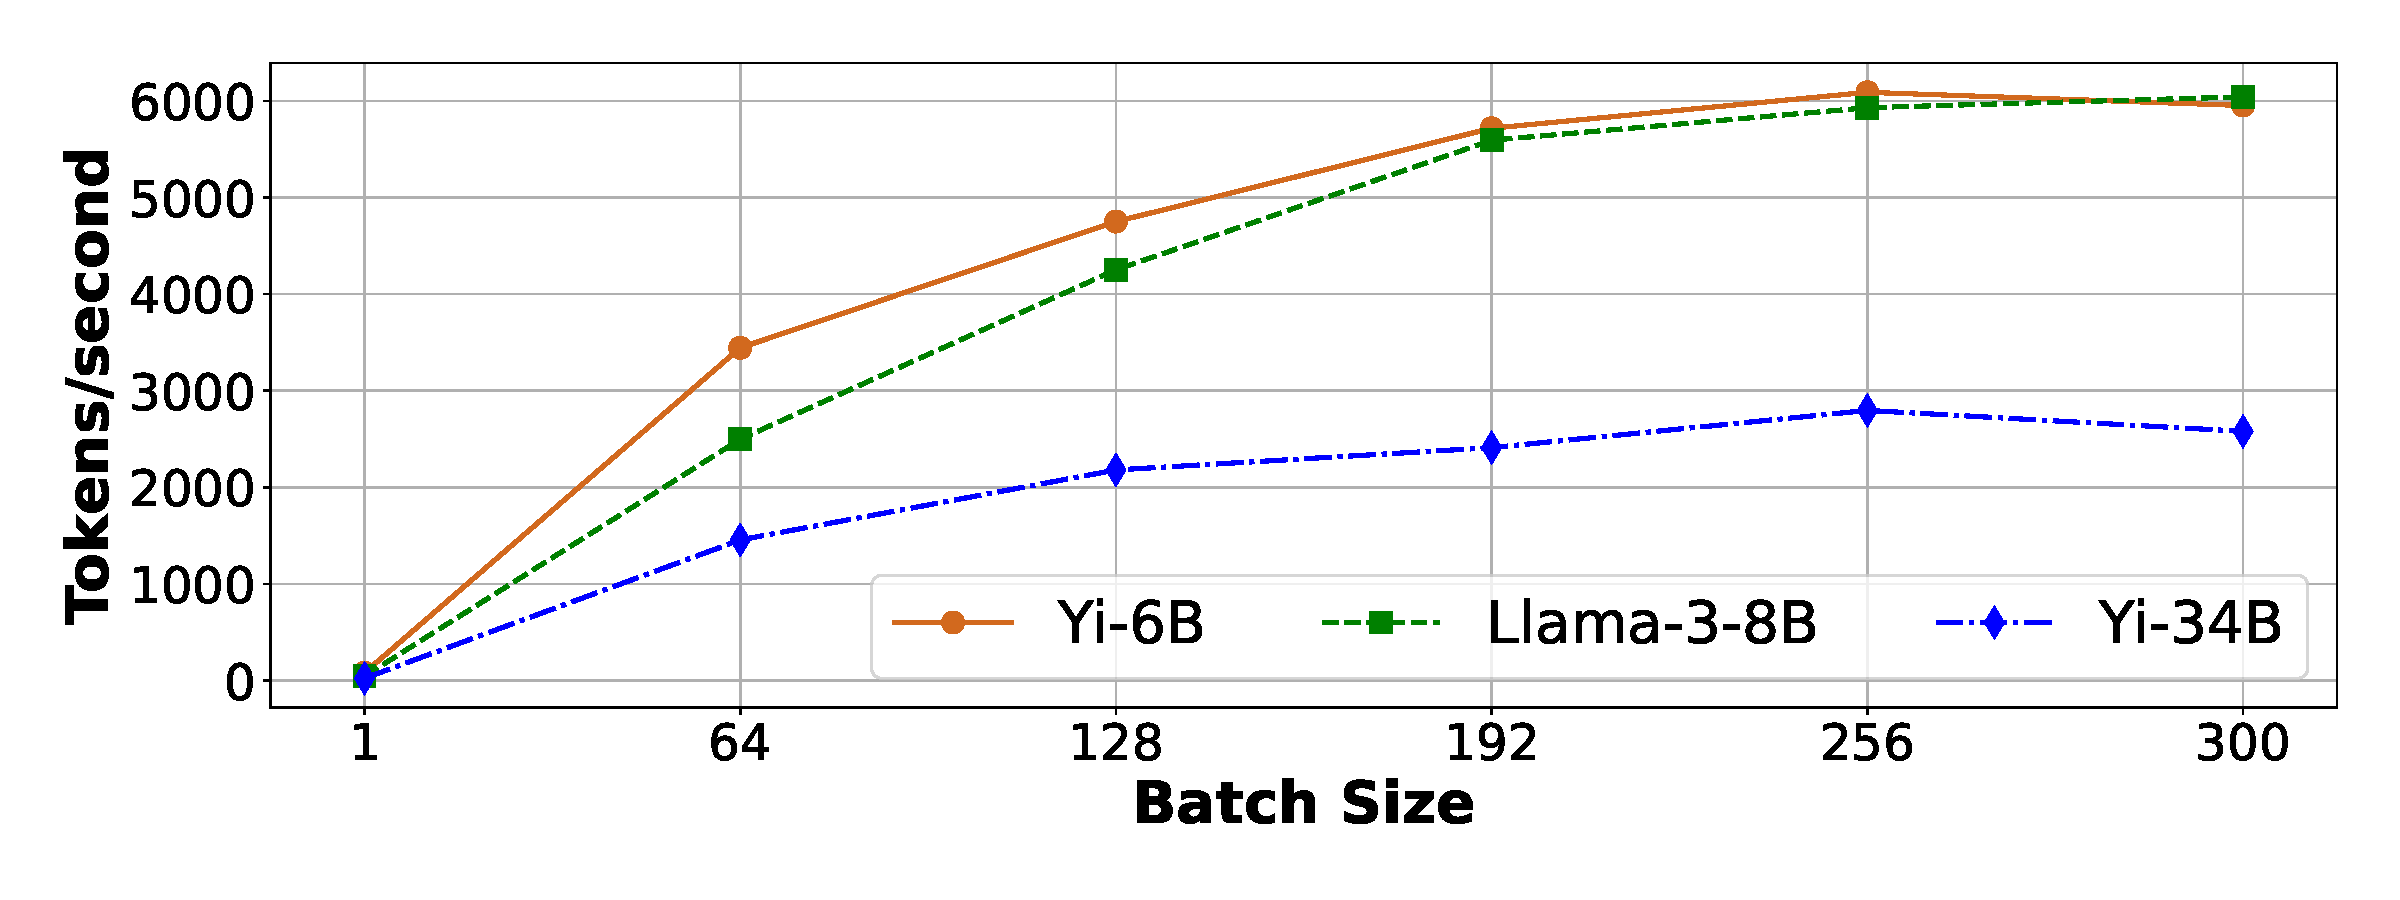
\includegraphics[trim={20 25 0 0}, clip=True, width=\textwidth]{graphs/figure_4_throughput.pdf}
        \caption{Decode throughput.}
        \label{fig:analysis:llm:memory:top}
    \end{subfigure}
    \\
    \begin{subfigure}[b]{0.9\columnwidth}
    \centering
        %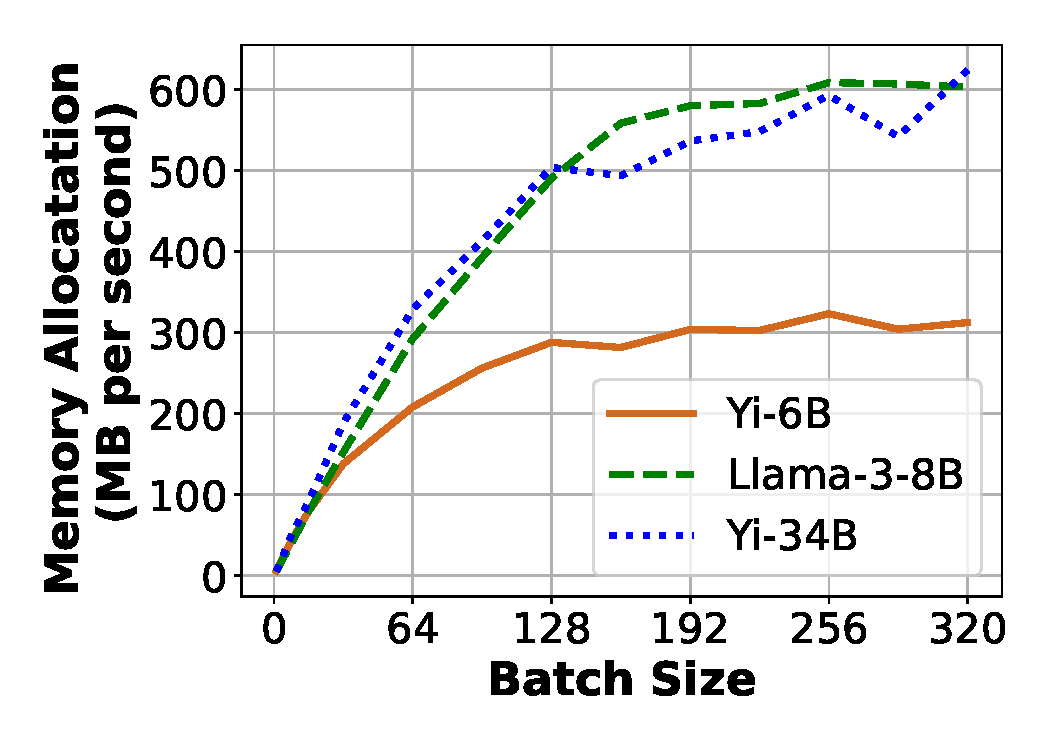
\includegraphics[trim={0 25 0 0}, clip=True, width=\textwidth]{graphs/analysis_decode_throughput/analysis_allocation_rate.pdf}
        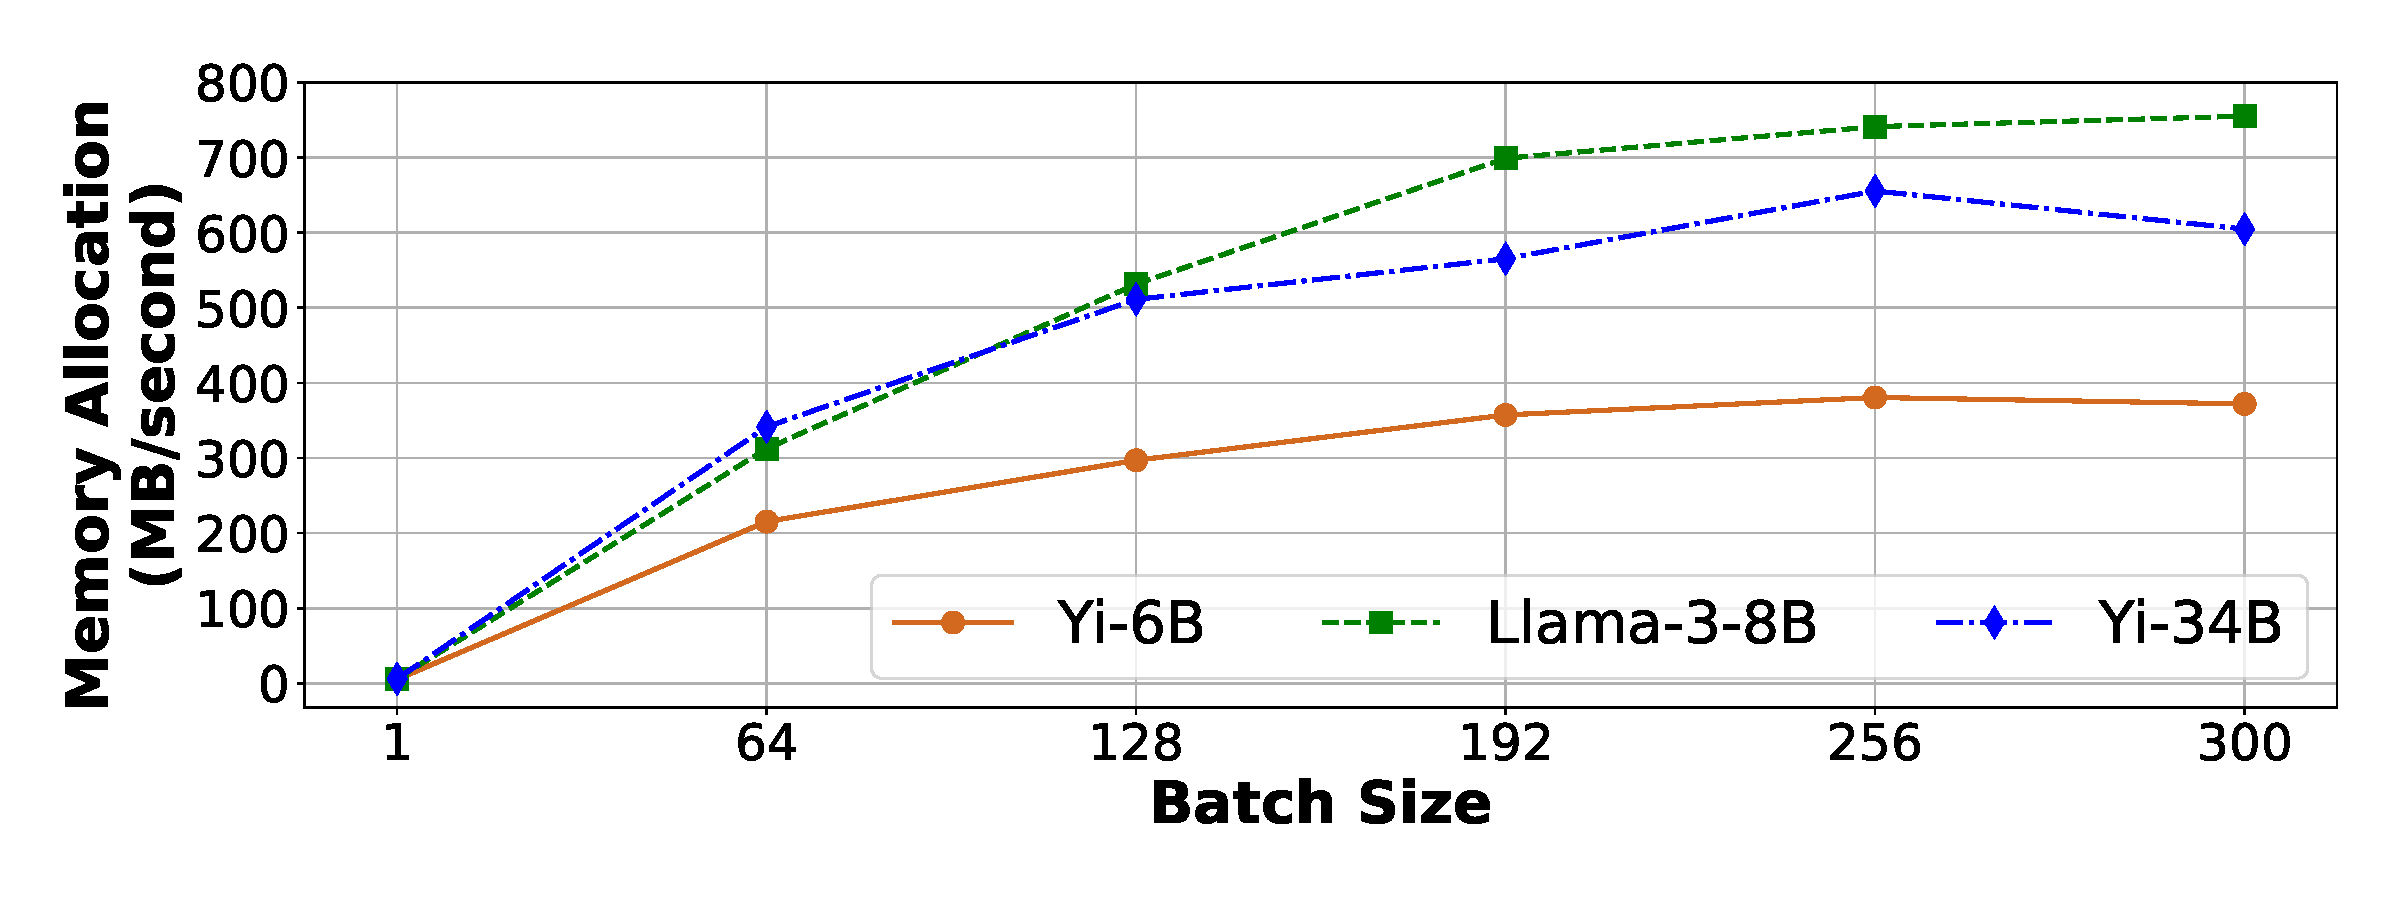
\includegraphics[trim={20 25 0 0}, clip=True, width=\textwidth]{graphs/figure_4_alloc_rate.pdf}
        \caption{Rate of memory allocation.}
        \label{fig:analysis:llm:memory:bottom}
    \end{subfigure}
    \caption{Decode throughput (top) and the rate of physical memory allocation (bottom) saturate at large batch sizes.}
    \label{fig:analysis:llm:memory}
\end{figure}

\begin{figure*}[t!]
    \centering
    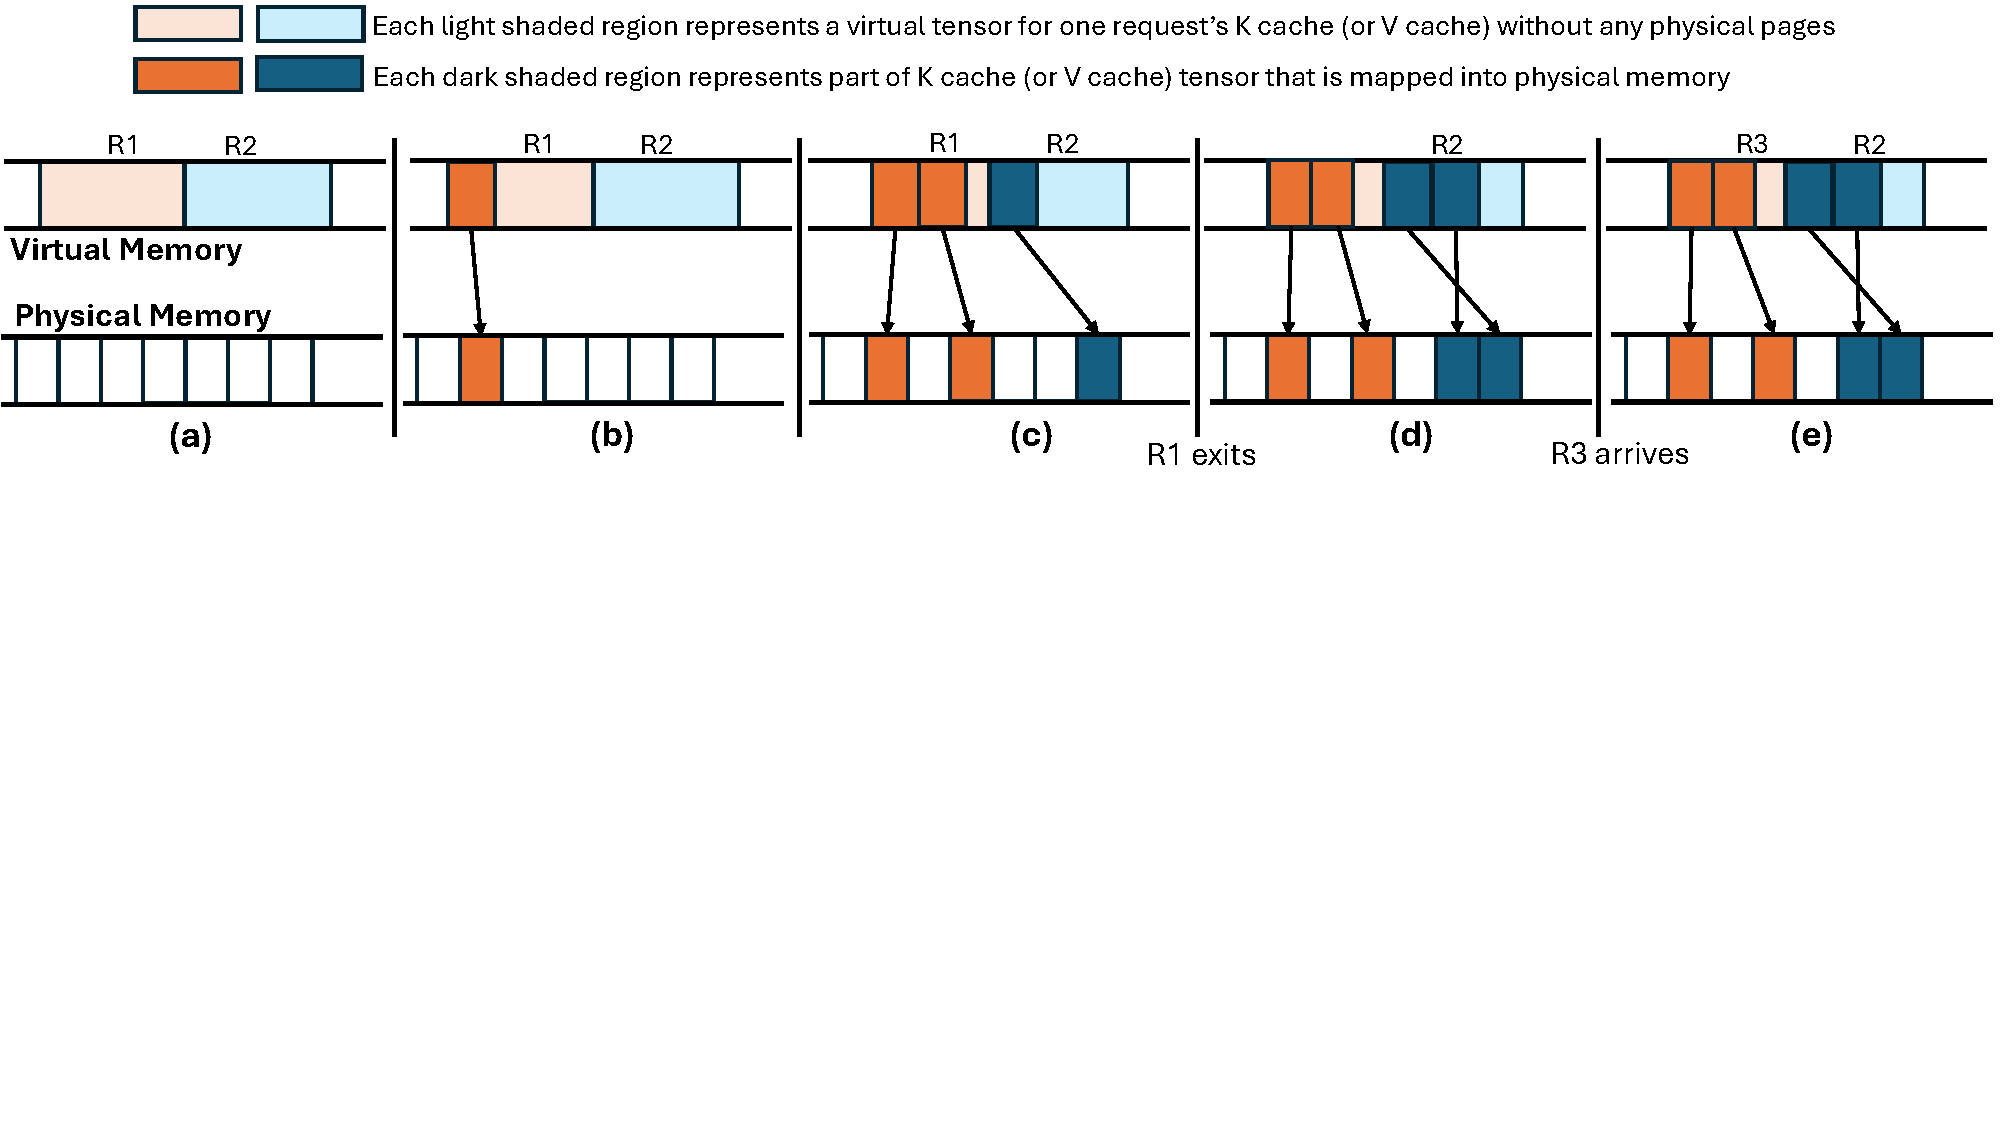
\includegraphics[trim={0 315 0 0}, clip=True, width=0.9\textwidth]{figures/vattention.pdf}
    \caption{Dynamic memory management in \sysname for a single \kcache (or \vcache) tensor. (a) shows a virtual tensor for a batch of two requests with no physical memory allocation yet. (b) \texttt{R1} is allocated one physical page. (c) \texttt{R1} is allocated two pages and \texttt{R2} is allocated one page. (d) \texttt{R1} has completed but \sysname does not reclaim its memory (deferred reclamation). (e) when \texttt{R3} arrives, \sysname assigns \texttt{R1}'s tensor to it which is already backed by physical memory. }
    \label{fig:design:vattention}
\end{figure*}


%In \sysname, we leverage these observations to implement an efficient dynamic memory management system for \kvcache. In the next section, we begin with a high-level deisgn overview of \sysname (\autoref{sec:design:overview}), then discuss how \sysname is used for serving LLMs (\autoref{sec:design:serving-llms}) and finally describe our optimizations (\autoref{sec:design:optimizations}).


